\chapter{Two Routes to the Gap}\label{ch:routeA}

Chapter~\ref{ch:positivity} showed that reflection positivity gives every gauge invariant observable a nonnegative spectral measure, and equipped us with the Thorin toolkit. This chapter turns that positivity into the mass gap in two ways, and then tests both on models where the gap can be computed. Route A translates the mass gap\index{mass gap} into the language of generalized gamma convolution\index{generalized gamma convolution}s\cite{Th77,Bo92}: the spectral measure\index{spectral measure} of a gauge invariant observable, after the Euclidean offset, is itself a Thorin measure\index{Thorin measure}, and the gap becomes the exponential tail index of the associated GGC. Route B (Section~\ref{ch:routeB}) places the spectrum on the L\'evy side and uses the $2\sin^2$ lemma to transport it to a Thorin density, so that the gap becomes an exact decay rate. Section~\ref{ch:examples} then tests the two dictionaries on the Ising chain, a massless field and the two dimensional Ising model.

\section{Route A: The Spectrum as a Thorin Measure}\label{sec:routeAmain}

Route A is the more direct of the two translations.

\subsection{The Yang Mills GGC}

Fix a gauge invariant observable $O$ with spectral measure $\mu$, gap $\Delta=\inf\operatorname{supp}\mu>0$, and an offset $\alpha>\alpha_0$. The Laplace transform of the offset correlation is the Stieltjes function\index{Stieltjes function}
\[
\widehat C_\alpha(s)=\int_0^\infty e^{-sr}\,C(\alpha+r)\,\mathrm dr=\int\frac{\mu_\alpha(\mathrm dE)}{s+E},\qquad \mu_\alpha=e^{-\alpha E}\mu .
\]
Physically, $\widehat C_\alpha$ is the zero momentum propagator of $O$ in a Laplace energy variable. Comparing with the logarithmic derivative of a GGC suggests integrating it.

\begin{proposition}[the Yang Mills GGC]\label{prop:ymggc}
The function
\[
\varphi_\alpha(s)=\exp\Big(-\int_0^s\widehat C_\alpha(r)\,\mathrm dr\Big)=\exp\Big(-\int\log\big(1+\tfrac sE\big)\mu_\alpha(\mathrm dE)\Big)
\]
is the Laplace transform of a GGC $X_\alpha$ with Thorin measure $\mu_\alpha$.
\end{proposition}

\begin{proof}
The two expressions agree because $\frac{\mathrm d}{\mathrm ds}\log(1+s/E)=1/(s+E)$ and both vanish at $s=0$. The Thorin conditions hold: $\mu_\alpha$ vanishes on $(0,\Delta)$, so the condition at the origin is trivial, and $\int_{(1,\infty)}E^{-1}\mu_\alpha(\mathrm dE)\le\int e^{-\alpha E}\mu(\mathrm dE)=C(\alpha)<\infty$.
\end{proof}

Simple spectra show the construction. If $\mu_\alpha=w\,\delta_m$ is a single stable particle of mass $m$ with weight $w$, then $X_\alpha$ is gamma distributed with shape $w$ and rate $m$. If the spectrum is a finite set of stable states, $X_\alpha$ is a sum of independent gamma variables, one per state, with shapes equal to the offset residues and rates equal to the masses. A continuous spectrum above a threshold contributes a continuous Thorin density\index{Thorin density}, and by Bondesson\index{Bondesson, L.}'s representation\cite{Bo92} an infinite shot noise of gamma process jumps, rescaled by rates equal to the multiparticle energies. Precisely, $X_\alpha=\sum_jY_j/E_j$, where $(E_j,Y_j)$ are the points of a Poisson process on $(0,\infty)^2$ with intensity $\mu_\alpha(\mathrm dE)\,y^{-1}e^{-y}\mathrm dy$.

\subsection{The gap is the tail index}

\begin{theorem}[gap as exponential moment threshold]\label{thm:abscissaB}
$\E e^{\lambda X_\alpha}<\infty$ for $\lambda<\Delta$, and $\E e^{\lambda X_\alpha}=\infty$ for $\lambda>\Delta$. Equivalently, the abscissa of convergence of $\varphi_\alpha$ is $-\Delta$, and the left edge of the Thorin support is the gap.
\end{theorem}

\begin{proof}
For $\lambda<\Delta$, the function $\log(1-\lambda/E)$ is bounded on $[\Delta,\infty)$ and of order $\lambda/E$ at infinity, so $\int\log(1-\lambda/E)\mu_\alpha(\mathrm dE)$ converges. By Campbell's theorem for the Poisson representation of Section~\ref{sec:routeAmain}, $\E e^{\lambda X_\alpha}=\exp\big(\int\!\!\int(e^{\lambda y/E}-1)y^{-1}e^{-y}\mathrm dy\,\mu_\alpha(\mathrm dE)\big)=\exp\big(-\int\log(1-\lambda/E)\,\mu_\alpha(\mathrm dE)\big)=\varphi_\alpha(-\lambda)<\infty$.

Suppose now that $\E e^{\lambda X_\alpha}<\infty$ for some $\lambda>\Delta$. A Laplace transform of a positive measure is analytic in the open half plane to the right of its abscissa, so $\varphi_\alpha$ is analytic on $\operatorname{Re}s>-\lambda$, a region containing a complex disc $N$ centred at $-\Delta$. Since $\varphi_\alpha(-\Delta)=\E e^{\Delta X_\alpha}>0$, after shrinking $N$ the function $\log\varphi_\alpha$ is analytic on $N$. On the part of $N$ off the negative real axis, $(\log\varphi_\alpha)'=-\widehat C_\alpha$, where $\widehat C_\alpha(s)=\int(s+E)^{-1}\mu_\alpha(\mathrm dE)$ is the Stieltjes transform. Hence $\widehat C_\alpha$ continues analytically across the segment $N\cap(-\infty,-\Delta]$ of its cut. By Stieltjes inversion, $\mu_\alpha$ then gives no mass to $\{E>\Delta:-E\in N\}$. An atom at $\Delta$ is also excluded, since it would make $-\Delta$ a pole of $\widehat C_\alpha$. This contradicts $\Delta\in\operatorname{supp}\mu_\alpha$.
\end{proof}

\begin{corollary}
$\liminf_{x\to\infty}\,-x^{-1}\log\Pr(X_\alpha>x)=\Delta$.
\end{corollary}

\begin{proof}
For a nonnegative random variable, Chebyshev's inequality gives $\Pr(X>x)\le e^{-\lambda x}\E e^{\lambda X}$, so $\liminf-x^{-1}\log\Pr(X>x)\ge\Delta$. Conversely, if the liminf exceeded $\Delta$, summation by parts would make $\E e^{\lambda X}$ finite for some $\lambda>\Delta$, contradicting Theorem~\ref{thm:abscissaB}. For a general random variable this gives only the liminf, since the tail may be irregular along a sparse sequence; that the limit exists for a GGC needs the GGC structure and is not proved here.
\end{proof}

The mass gap is therefore the exponential moment threshold of the Yang Mills GGC, and its tail index in the liminf sense of the corollary. In Bondesson's shot noise picture this is transparent: the variable is a sum of gamma process jumps rescaled by rates drawn from the spectrum, and the exponential moments are governed by the slowest rate, which is the lightest state.

\begin{figure}[t]
\centering
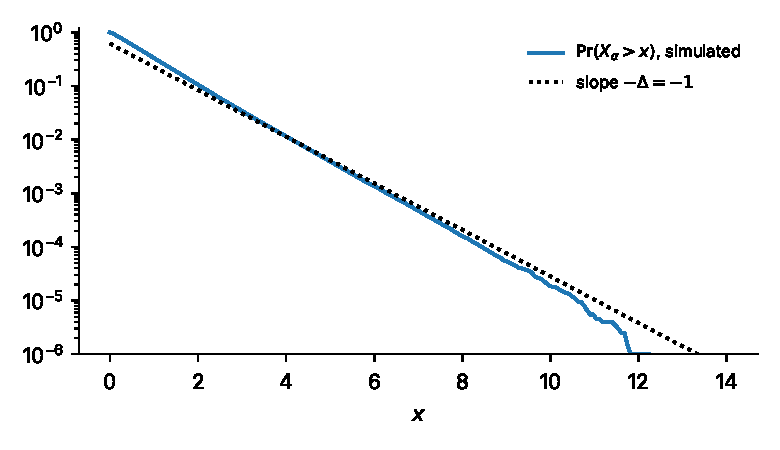
\includegraphics[width=0.92\textwidth]{figures/routeA_tail.pdf}
\caption[Route A for a toy spectrum: stable states at $1,1.5,1.9$ and a continuum from $2$, offset $\alpha=1/2$]{Route A for a toy spectrum: stable states at $1,1.5,1.9$ and a continuum from $2$, offset $\alpha=1/2$. Two million samples of the Yang Mills GGC were drawn, each a sum of independent gamma variables, one per Thorin atom, with the continuum discretised into 3000 atoms. The log tail is asymptotically linear with slope $-\Delta=-1$; the fitted slope over the visible range is $-1.06$, steeper because of the polynomial factor $x^{w-1}$ contributed by the lightest atom.}
\label{fig:routeAtail}
\end{figure}

\subsection{The Clay statement in Route A language}

The problem asks for a single $\Delta>0$ that bounds the gaps of all gauge invariant observables in the continuum theory. In Route A language this reads as follows.

\begin{quote}
For every gauge invariant observable $O$, the Yang Mills GGC $X_{O,\alpha}$ has $\E e^{\lambda X_{O,\alpha}}<\infty$ for all $\lambda<\Delta$.
\end{quote}

The continuum theory is a limit of lattice theories, and the following closure property shows what is needed.

\begin{proposition}\label{prop:closureA}
Let $\mu^{(a)}_\alpha$ be offset lattice spectral measures, in physical units, converging weakly to $\mu_\alpha$ as $a\to0$. If $\Delta_0>0$ and $\operatorname{supp}\mu^{(a)}_\alpha\subset[\Delta_0,\infty)$ for all $a$, then $\operatorname{supp}\mu_\alpha\subset[\Delta_0,\infty)$, and the GGC laws $X^{(a)}_\alpha$ converge weakly to $X_\alpha$.
\end{proposition}

\begin{proof}
The set of measures supported in the closed set $[\Delta_0,\infty)$ is closed under weak convergence. For each $s\ge0$ the function $E\mapsto\log(1+s/E)\le s/\Delta_0$ is bounded and continuous on $[\Delta_0,\infty)$, so weak convergence of the Thorin measures gives convergence of the Laplace transforms $\varphi^{(a)}_\alpha(s)$, hence weak convergence of the GGC laws.
\end{proof}

So a lattice gap that is uniform in the spacing, measured in physical units, passes to the limit. The difficulty, which no closure property can remove, is proving that uniformity.

\subsection{What Route A adds}

Route A is a change of language; its value is what the language brings. First, GGCs are closed under convolution, so independent sectors combine by convolving their GGCs and the gap of the combination is the minimum of the gaps. Second, Bondesson's shot noise representation\cite{Bo92} makes spectral quantities simulable; in the Riemann setting the candidate Thorin measure is not known to be positive and the shot noise may not exist, but here it always does. Third, the singularity of $\varphi_\alpha$ nearest the origin sits at $-\Delta$, which is the K\"all\'en Lehmann statement that the spectral density vanishes below the first threshold.

Route A gives no mechanism for keeping the support away from zero. That needs a parameter that can be driven to infinity. The Euclidean offset $\alpha$ is that parameter, and the $2\sin^2$ lemma of Route B (Section~\ref{ch:routeB}) exploits it.

\section{Route B: The 2 sin\texorpdfstring{$^2$}{2} Lemma and L\'evy Exponents}\label{ch:routeB}

Route A placed the spectrum on the Thorin side of a GGC. Route B places it on the L\'evy side, and uses the lemma at the centre of our Riemann programme\cite{PS26a} to transport it to a Thorin density\index{Thorin density}. The result is a family of Thorin densities indexed by Euclidean time, and the gap becomes their exact rate of decay.

\subsection{The lemma}

\begin{lemma}[the Polson $2\sin^2$ lemma]\label{lem:2sin2B}
For $x,w>0$ and $u=w^2/2$,
\[
e^{-wx}+wx-1=\int_0^\infty\log\Big(1+\frac uz\Big)\,k_x(z)\,\mathrm dz,
\]
where
\[
k_x(z)=\frac{x}{\pi\sqrt{2z}}\;2\sin^2\!\big(x\sqrt{z/2}\big)\ge0 .
\]
\end{lemma}

\begin{proof}
Substitute $z=2y^2$, so $\mathrm dz=4y\,\mathrm dy$ and $\sqrt{2z}=2y$. The right side becomes
\[
\frac{4x}{\pi}\int_0^\infty\sin^2(xy)\,\log\Big(1+\frac{a^2}{y^2}\Big)\mathrm dy,\qquad a=\frac w2 .
\]
Write $\sin^2(xy)=\frac12(1-\cos2xy)$ and use the two classical integrals
\[
\int_0^\infty\log\Big(1+\frac{a^2}{y^2}\Big)\mathrm dy=\pi a,
\]
\[
\int_0^\infty\log\Big(1+\frac{a^2}{y^2}\Big)\cos(2xy)\,\mathrm dy=\frac{\pi}{2x}\big(1-e^{-2ax}\big).
\]
The right side equals $\frac{4x}{\pi}\cdot\frac12\big(\pi a-\frac{\pi}{2x}(1-e^{-2ax})\big)=wx-1+e^{-wx}$.
\end{proof}

The left side is the compensated Laplace exponent of a single jump of size $x$; the right side is a Thorin integral with a nonnegative density. Integrating against a nonnegative L\'evy measure therefore produces a nonnegative Thorin measure\index{Thorin measure}. In the Riemann programme the relevant L\'evy measure, built from the primes, is signed inside the critical strip, and positivity of the transported Thorin measure is tied to the absence of zeros in a region, as developed in the Riemann volumes\cite{PS26a}; nothing here depends on that statement. In Yang Mills the L\'evy measure is the spectral measure\index{spectral measure}, and it is nonnegative by reflection positivity\index{reflection positivity}.

\subsection{The compensated increment}

Integrate the lemma against $\mu_\alpha(\mathrm dE)/E$ with $x=E$:
\[
L_\alpha(w)=\int\big(e^{-wE}+wE-1\big)\frac{\mu_\alpha(\mathrm dE)}{E}.
\]
Differentiating in $w$ gives $L_\alpha'(w)=\int(1-e^{-wE})\mu_\alpha(\mathrm dE)=C(\alpha)-C(\alpha+w)$, and $L_\alpha(0)=0$, so
\[
L_\alpha(w)=\int_0^w\big(C(\alpha)-C(\alpha+s)\big)\mathrm ds\ \ge0 .
\]
It is finite because $e^{-wE}+wE-1\le wE$. In words, $L_\alpha(w)$ is the area between the flat line at height $C(\alpha)$ and the decaying correlation over the window $[\alpha,\alpha+w]$.

\subsection{The Thorin density is a L\'evy exponent}

\begin{theorem}\label{thm:thorinB}
For $\alpha>\alpha_0$, the function $u\mapsto\exp\big(-L_\alpha(\sqrt{2u})\big)$ is the Laplace transform of a GGC whose Thorin measure has density
\[
T_\alpha(z)=\frac{\psi_\alpha(t)}{\pi t},\qquad t=\sqrt{2z},
\]
where
\[
\psi_\alpha(t)=\int(1-\cos tE)\,\mu_\alpha(\mathrm dE)=C(\alpha)-\operatorname{Re}C(\alpha+it)
\]
is the L\'evy exponent\index{Levy exponent@L\'evy exponent} of the symmetric compound Poisson process whose jump measure is $\mu_\alpha$ symmetrised (jumps $\pm E$, each with weight $\frac12\mu_\alpha(\mathrm dE)$).
\end{theorem}

\begin{proof}
All integrands are nonnegative, so Tonelli's theorem allows the exchange of the $E$ and $z$ integrals. Lemma~\ref{lem:2sin2B} gives the Thorin representation with density $\int k_E(z)\mu_\alpha(\mathrm dE)/E$, and $x\sqrt{z/2}=tE/2$ together with $2\sin^2(tE/2)=1-\cos tE$ gives the stated form. The Thorin conditions hold because $\psi_\alpha\le2C(\alpha)$, so $T_\alpha(z)=O(z^{-1/2})$ at infinity, and $\psi_\alpha(t)\sim\frac12m_2t^2$ as $t\to0$ with $m_2=\int E^2\mu_\alpha(\mathrm dE)<\infty$.
\end{proof}

The theorem has a direct quantum mechanical meaning. Let $\Psi=e^{-\alpha H/2}O\Omega$ be the state obtained by evolving the observable for Euclidean time $\alpha/2$. Then
\[
C(\alpha+it)=\langle\Psi,e^{-itH}\Psi\rangle,
\]
the return amplitude of $\Psi$ after real time $t$. So $\psi_\alpha(t)/C(\alpha)$ is the deficit $1-\operatorname{Re}\langle\Psi,e^{-itH}\Psi\rangle/\|\Psi\|^2$ of the normalised return amplitude. Nonnegativity of the Thorin density is the Cauchy and Schwarz inequality $|\langle\Psi,e^{-itH}\Psi\rangle|\le\|\Psi\|^2$. The Thorin variable $z$ is real time in disguise, through $t=\sqrt{2z}$.

The parallel with the Riemann programme is exact enough to tabulate.
\begin{center}
\small
\begin{tabular}{lll}
\toprule
 & reciprocal Xi & Yang Mills \\ \midrule
L\'evy side & primes, jumps $\log p$ & spectrum, jumps $E$ \\
Thorin side & zero ordinates, $\gamma=\sqrt{2z}$ & real time, $t=\sqrt{2z}$ \\
level parameter & abscissa $\alpha$ & Euclidean time $\alpha$ \\
positivity of $T_\alpha$ & open in the strip & Cauchy and Schwarz \\
hard question & is $T_\alpha\ge0$? & how fast does $T_\alpha$ decay? \\
\bottomrule
\end{tabular}
\end{center}

\subsection{The gap is the decay rate}

\begin{theorem}[gap as Thorin decay rate]\label{thm:rateB}
Let $\Delta=\inf\operatorname{supp}\mu$.
\begin{enumerate}
\item[(i)] For all $z>0$ and $\alpha\ge\alpha'>\alpha_0$, $T_\alpha(z)\le e^{-\Delta(\alpha-\alpha')}T_{\alpha'}(z)$.
\item[(ii)] For all but countably many $z$, $\lim_{\alpha\to\infty}-\alpha^{-1}\log T_\alpha(z)=\Delta$.
\item[(iii)] For each $z$ with $T_\alpha(z)>0$, $\alpha\mapsto\log T_\alpha(z)$ is convex, so the local rate $r_\alpha(z)=-\partial_\alpha\log T_\alpha(z)$ is nonincreasing, and for $z$ outside the exceptional countable set of (ii) it decreases to $\Delta$.
\end{enumerate}
\end{theorem}

\begin{proof}
(i) On the support, $e^{-\alpha E}=e^{-(\alpha-\alpha')E}e^{-\alpha' E}\le e^{-(\alpha-\alpha')\Delta}e^{-\alpha' E}$, and the kernel $1-\cos tE$ is nonnegative.

(ii) The bound (i) gives $\liminf-\alpha^{-1}\log T_\alpha(z)\ge\Delta$. For the reverse inequality, $q_t(E)=1-\cos tE$ vanishes only on the lattice $2\pi\Z/t$. Only countably many values of $t$ place one of the countably many atoms of $\mu$ on that lattice, and the continuous part of $\mu$ gives zero mass to every countable set. For any other $t$ and any $\varepsilon>0$, $c=\int_{[\Delta,\Delta+\varepsilon]}q_t\,\mathrm d\mu>0$, and $T_\alpha(z)\ge(\pi t)^{-1}c\,e^{-\alpha(\Delta+\varepsilon)}$.

(iii) $T_\alpha(z)$ is, as a function of $\alpha$, the Laplace transform of the nonnegative measure $(\pi t)^{-1}q_t(E)\mu(\mathrm dE)$, hence log convex by H\"older's inequality. A log convex function whose logarithm decays at rate $\Delta$ has local rate decreasing to $\Delta$.
\end{proof}

Part (iii) repeats the lesson of Proposition~\ref{prop:logconvex}: every local rate computed from data bounds the gap from above.

\begin{figure}[t]
\centering
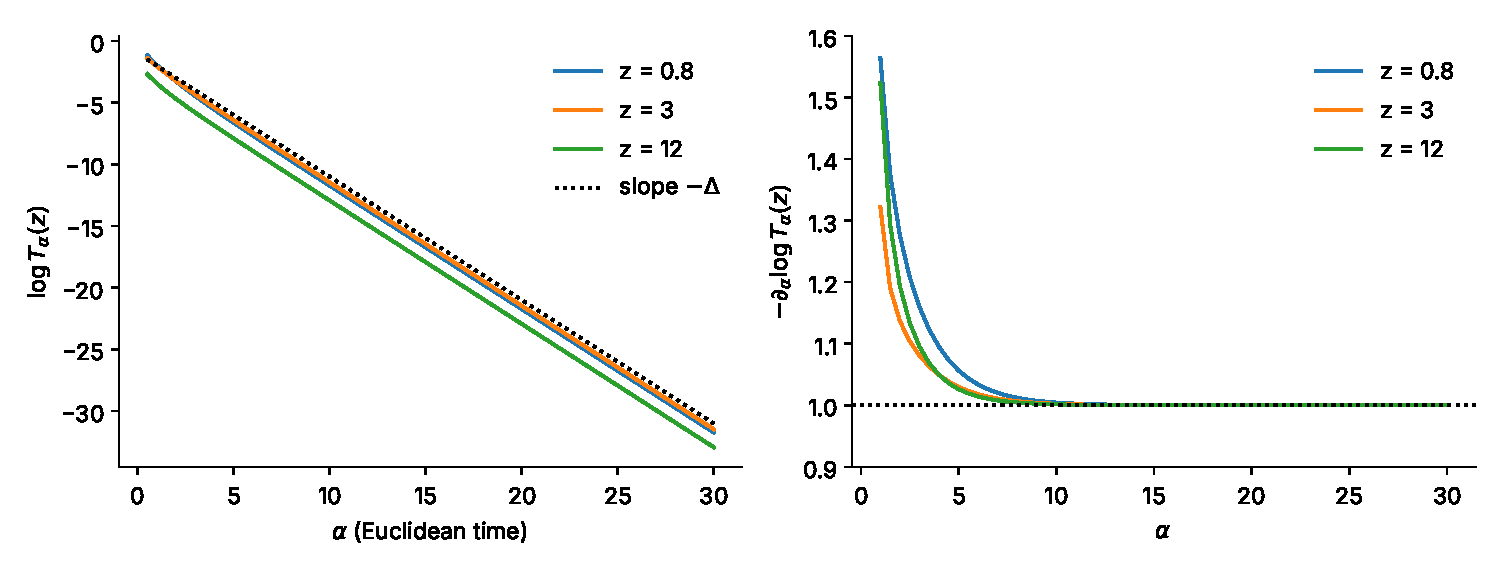
\includegraphics[width=\textwidth]{figures/thorin_gap.pdf}
\caption[Route B for the toy spectrum of Figure~\ref{fig:routeAtail}. Left: $\log T_\alpha(z)$ against]{Route B for the toy spectrum of Figure~\ref{fig:routeAtail}. Left: $\log T_\alpha(z)$ against Euclidean time for three values of $z$. Right: the local rates decrease monotonically to the gap $\Delta=1$. The real time formula of Theorem~\ref{thm:thorinB} agrees with the direct integral to ten digits; the two integrands are algebraically identical, so this checks the numerical evaluation only.}
\label{fig:thorinB}
\end{figure}

\subsection{The constant is free}

The continuum problem concerns a family of measures $\mu^{(a)}$ indexed by the lattice spacing. The natural uniform statement in Route B is an inequality between Thorin densities, and its constant carries no information.

\begin{theorem}[equivalences]\label{thm:equivB}
Let $\{\mu^{(a)}\}$ be nonnegative measures on $(0,\infty)$ with $\sup_a\int e^{-\alpha_0E}\mu^{(a)}(\mathrm dE)<\infty$, and let $m>0$. The following are equivalent.
\begin{enumerate}
\item[(a)] $\operatorname{supp}\mu^{(a)}\subset[m,\infty)$ for every $a$.
\item[(b)] There are $M'$ and $\tau_0$ with $C^{(a)}(\tau)\le M'e^{-m\tau}$ for all $\tau\ge\tau_0$ and all $a$.
\item[(c)] There is $M<\infty$ with $T^{(a)}_\alpha(z)\le Me^{-m(\alpha-\alpha')}T^{(a)}_{\alpha'}(z)$ for all $a$, all $z$ and all $\alpha\ge\alpha'>\alpha_0$.
\item[(d)] Statement (c) holds with $M=1$.
\end{enumerate}
\end{theorem}

\begin{proof}
(a) implies (d) by Theorem~\ref{thm:rateB}(i), and (d) implies (c) trivially. If (c) holds, then for fixed $a$ and $\alpha'$ the decay rate of $T^{(a)}_\alpha(z)$ is at least $m$, and Theorem~\ref{thm:rateB}(ii) gives (a). Finally (a) and (b) are equivalent by Proposition~\ref{prop:gapdecay}, whose constants are uniform under the hypothesis.
\end{proof}

We call (c) the uniform Thorin gap inequality. The theorem says that it is exactly a uniform spectral gap, that it can always be stated with $M=1$, and that it is equivalent to uniform exponential decay of correlations. Combining with weak convergence gives the continuum statement.

\begin{corollary}[continuum]\label{cor:continuumB}
If lattice measures in physical units have offset measures $e^{-\alpha_0E}\mu^{(a)}$ converging weakly, and satisfy the uniform Thorin gap inequality with one $m=\Delta_0$, then the continuum theory has a gap of at least $\Delta_0$.
\end{corollary}

\begin{proof}
For $\alpha>\alpha_0$ the kernel $e^{-(\alpha-\alpha_0)E}(1-\cos tE)$ is bounded and continuous in $E$, so $T^{(a)}_\alpha(z)\to T_\alpha(z)$ pointwise. The inequality passes to the limit, and Theorem~\ref{thm:rateB}(ii) applies.
\end{proof}

\subsection{Correlators are not themselves GGC}

Is the normalised correlation $C(\alpha+\tau)$ itself a GGC in the variable $\tau$, or even HCM? It is not, as soon as the spectrum has two isolated levels.

\begin{proposition}\label{prop:notggcB}
If $\int_0^\infty C(\alpha+s)\,\mathrm ds<\infty$ and $\mu$ has atoms at $E_1<E_2$ with $\mu((E_1,E_2))=0$, then the probability density proportional to $C(\alpha+\tau)$ is not a GGC, and hence not HCM.
\end{proposition}

\begin{proof}
Its Laplace transform is proportional to $\widehat p(s)=\int\mu_\alpha(\mathrm dE)/(E+s)$. On the interval $(-E_2,-E_1)$ the function $\widehat p$ is real analytic and strictly decreasing, since $\widehat p'(s)=-\int(E+s)^{-2}\mu_\alpha(\mathrm dE)<0$, and it runs from $+\infty$ near $-E_2$ to $-\infty$ near $-E_1$. It therefore vanishes at some $-\zeta$ with $E_1<\zeta<E_2$. If the density were a GGC with Thorin measure $U$, then $-(\log\widehat p)'=\int U(\mathrm dt)/(s+t)$ would be a Stieltjes function\index{Stieltjes function}. But near $-\zeta$ the function $-\widehat p'/\widehat p$ is meromorphic with a simple pole of residue $-1$, and Stieltjes inversion then gives $U=-\delta_\zeta$ near $\zeta$, which is negative. HCM laws are GGC, so the density is not HCM either.
\end{proof}

For the toy spectrum of Figure~\ref{fig:routeAtail}, including its continuum, at offset $\alpha=1/2$ the negative Thorin atoms sit at $1.3216$ and $1.8208$ (\texttt{code/op1\_checks.py}). In lattice SU(3) the scalar channel has two stable states below the two glueball\index{glueball} threshold\cite{MP}, so that channel is not a GGC in Euclidean time. This is why both Routes A and B build their GGCs indirectly, by integrating a Stieltjes function or by transporting a L\'evy measure, rather than asking the correlation itself to be a GGC.

\section{Models Where the Gap Can Be Computed}\label{ch:examples}

Before moving on, we test the two dictionaries on models where the spectrum is known exactly. The examples are chosen to show three behaviours: a gap that survives a renormalization flow, no gap at all, and a gap that closes at a critical point. Yang Mills is expected to behave like the first, and the contrast with the other two clarifies what the uniform Thorin gap inequality does and does not demand.

\subsection{The Ising chain and exact decimation}

The one dimensional Ising\index{Ising model} model with coupling $K$ has spins $\sigma_i=\pm1$ and weight $\exp(K\sum_i\sigma_i\sigma_{i+1})$. Its transfer matrix\index{transfer matrix} $\begin{pmatrix}e^K&e^{-K}\\ e^{-K}&e^K\end{pmatrix}$ has eigenvalues $2\cosh K$ and $2\sinh K$, and the spin correlation is
\[
\langle\sigma_0\sigma_n\rangle=(\tanh K)^n=e^{-n\,m(K)},\qquad m(K)=-\log\tanh K .
\]
The spectral measure\index{spectral measure} of the spin observable is a single atom at $m(K)$, so in Route A the GGC $X_\alpha$ is a gamma variable with rate $m(K)$, and in Route B the Thorin density\index{Thorin density} is a single damped oscillation. The gap is positive for every finite $K$, and it closes only at zero temperature, $K\to\infty$, where $m(K)\approx2e^{-2K}$ (Figure~\ref{fig:examplesgaps}).

The chain also has an exact renormalization group. Summing out every other spin gives a chain with coupling $K'$ satisfying
\[
\tanh K'=(\tanh K)^2,
\]
and more generally $\tanh K\mapsto(\tanh K)^b$ for decimation\index{decimation} by $b$. In the variable $u=\tanh K$ decimation is exactly $u\mapsto u^b$, the same form as the decimation of two dimensional Yang Mills in Chapter~\ref{ch:twod}, where character coefficients are raised to the power $b^2$. The resemblance is not an accident. Two dimensional $\Z_2$ lattice gauge theory is equivalent to a product of independent Ising chains, and the variable $u$ is the single nontrivial character coefficient of the plaquette weight. The correlation length $1/m(K)$, measured in lattice units, is divided by $b$ at each step, and the flow runs from any finite $K$ to $K=0$, the disordered fixed point. The continuum limit $K\to\infty$ requires the lattice spacing to shrink like $e^{-2K}$, and in those units the gap is constant. This is a toy version of asymptotic freedom\index{asymptotic freedom}.

\subsection{A massless field}

Next consider a theory with no gap. For a free massless field, or at a critical point, the zero momentum correlation of a suitable composite observable decays like a power, $C(\tau)\propto\tau^{-\kappa}$ for some $\kappa>0$. By Bernstein\index{Bernstein theorem}'s theorem~\cite{Be29} the spectral measure is
\[
\mu(\mathrm dE)=\frac{E^{\kappa-1}}{\Gamma(\kappa)}\,\mathrm dE,
\]
supported down to zero. In Route A the offset measure $e^{-\alpha E}E^{\kappa-1}\mathrm dE/\Gamma(\kappa)$ is a Thorin measure\index{Thorin measure} with no gap at the origin, and the Yang Mills GGC has $\E e^{\lambda X_\alpha}=\infty$ for every $\lambda>0$: its tail is heavier than any exponential. In Route B,
\[
\begin{aligned}
T_\alpha(z)&=\frac{1}{\pi t\,\Gamma(\kappa)}\int_0^\infty E^{\kappa-1}e^{-\alpha E}(1-\cos tE)\,\mathrm dE\\
&=\frac{1}{\pi t}\Big(\alpha^{-\kappa}-\operatorname{Re}(\alpha+it)^{-\kappa}\Big),
\end{aligned}
\]
which decays like a power of $\alpha$. The local rate $-\partial_\alpha\log T_\alpha(z)$ tends to zero like $(\kappa+2)/\alpha$ (Figure~\ref{fig:masslessrates}). No inequality of the form $T_\alpha\le Me^{-m(\alpha-\alpha')}T_{\alpha'}$ can hold with $m>0$. This is what the absence of a gap looks like in the Thorin language: the family of Thorin densities is still positive and still monotone, but its decay is polynomial.

\begin{figure}[t]
\centering
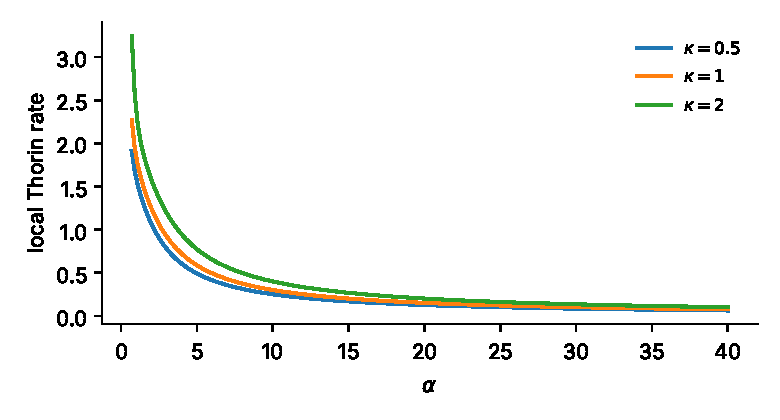
\includegraphics[width=0.92\textwidth]{figures/massless_rates.pdf}
\caption[Route B local Thorin rates for a massless spectrum $\mu(\mathrm dE)\propto E^{\kappa-1}\mathrm dE$,]{Route B local Thorin rates for a massless spectrum $\mu(\mathrm dE)\propto E^{\kappa-1}\mathrm dE$, with $t=1.3$ and $\kappa=0.5,1,2$. The rates decrease to zero like $(\kappa+2)/\alpha$; there is no gap.}
\label{fig:masslessrates}
\end{figure}

\subsection{The two dimensional Ising model}

The third example has a gap that closes at a critical point. For the two dimensional Ising model on the square lattice with coupling $K$, Onsager \cite{On44} and Kaufman \cite{Kau49} diagonalised the row to row transfer matrix. Define the dual coupling $K^*$ by $\tanh K^*=e^{-2K}$. The critical point is the self dual point $K_c=\frac12\log(1+\sqrt2)$, and the gap of the transfer matrix, in lattice units, is
\[
G(K)=2\,|K-K^*| .
\]
It is positive on both sides of $K_c$ and vanishes linearly at $K_c$, so the correlation length diverges like $|K-K_c|^{-1}$ (Figure~\ref{fig:examplesgaps}). For $K<K_c$ (high temperature) the connected spin spin correlation decays at rate $G(K)=2|K-K^*|$. For $K>K_c$ (low temperature) the spin couples first to a two particle state, so its spectral measure, the one Routes A and B see, starts at $2G(K)$, and the connected spin spin correlation decays at rate $4|K-K^*|$, twice the transfer matrix gap.

\begin{figure}[t]
\centering
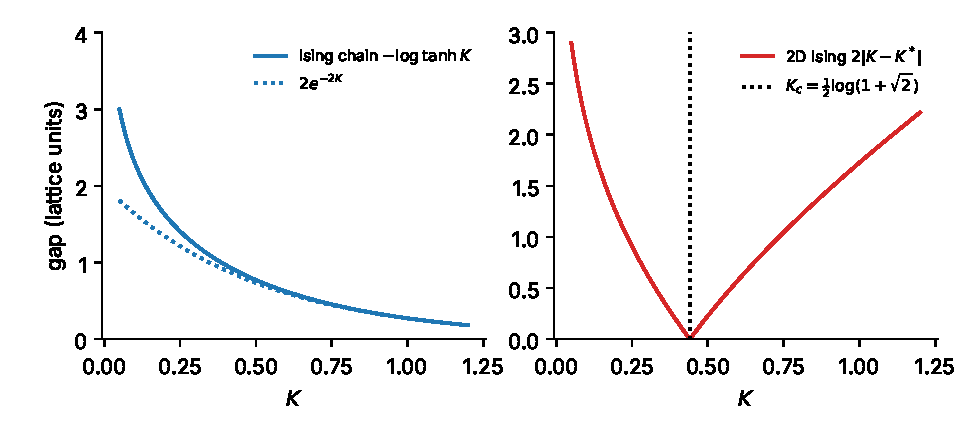
\includegraphics[width=\textwidth]{figures/examples_gaps.pdf}
\caption[Left: the Ising chain gap $-\log\tanh K$, positive for every finite $K$, closing only at zero]{Left: the Ising chain gap $-\log\tanh K$, positive for every finite $K$, closing only at zero temperature like $2e^{-2K}$. Right: the transfer matrix gap of the two dimensional Ising model, $2|K-K^*|$, which closes at the critical coupling; for $K>K_c$ the connected spin correlation decays at twice this rate.}
\label{fig:examplesgaps}
\end{figure}

Near $K_c$ the model has a continuum limit, the massive Ising field theory, obtained by letting the lattice spacing shrink like $|K-K_c|$. In those units the gap is again constant (for either of the two decay rates above), and the uniform Thorin gap inequality holds along that trajectory. At $K_c$ itself the continuum limit is the critical Ising field theory, a conformal field theory with no gap, and the Thorin densities decay polynomially as in the massless example.

\subsection{Lessons for Yang Mills}

The three examples sharpen what the Clay problem asks.
\begin{enumerate}
\item[(i)] In the two Ising examples a continuum limit exists, and the uniform Thorin gap inequality holds along it if and only if the correlation length in lattice units diverges no faster than the inverse lattice spacing. The inequality is not a property of a single lattice theory but of a trajectory.
\item[(ii)] In the Ising chain the continuum limit is reached at an endpoint of the coupling range, $K\to\infty$, and an exact renormalization map moves along the trajectory. Yang Mills is expected to behave this way, with $\beta\to\infty$ in place of $K\to\infty$ and asymptotic freedom fixing the rate. The Migdal Kadanoff ladder of Section~\ref{ch:mk} is the closest analogue in four dimensions.
\item[(iii)] In the two dimensional Ising model the continuum limit is reached at an interior critical point. Monte Carlo studies of lattice Yang Mills for SU(2)~\cite{Cr80} find no such transition in four dimensions, so the correlation length is expected to diverge only as $\beta\to\infty$. That is why the mass gap problem is a problem about the crossover between strong and weak coupling rather than about a critical point.
\item[(iv)] Absence of a gap shows up in Route A as a heavier than exponential tail of the GGC, and in Route B as polynomial decay of the Thorin densities. Both are detectable in principle, but by Proposition~\ref{prop:logconvex} data can only bound the gap from above, so a slowly decaying correlation can never be certified massless or massive by measurement alone.
\end{enumerate}

\section*{Exercises}
\begin{enumerate}
\item For $\mu_\alpha=w_1\delta_{m_1}+w_2\delta_{m_2}$, identify $X_\alpha$ as a sum of two independent gamma variables and verify Theorem~\ref{thm:abscissaB} directly.
\item Show that if $\mu$ has density $\rho(E)\sim c(E-\Delta)^\nu$ near $\Delta$, then $\Pr(X_\alpha>x)=e^{-\Delta x+o(x)}$, the full limit and not only the liminf of the corollary, by splitting off the part of $\mu_\alpha$ in $[\Delta,\Delta+\varepsilon]$ as an independent gamma convolution.
\item Show that the Yang Mills GGC of a direct sum of two independent sectors is the convolution of their GGCs, and that its gap is the minimum of the two gaps.
\item Use Bondesson's shot noise representation (the jumps $Y_j$ of a gamma process, intensity $y^{-1}e^{-y}\mathrm dy$, each divided by a rate $E_j$, the pairs $(E_j,Y_j)$ forming the Poisson process of Section~\ref{sec:routeAmain} with intensity $\mu_\alpha(\mathrm dE)\,y^{-1}e^{-y}\mathrm dy$) to write a simulation algorithm for $X_\alpha$ when $\mu_\alpha$ has an atomic part and a continuous part, and implement it for the toy spectrum of Figure~\ref{fig:routeAtail}.
\item Verify the two integrals used in the proof of Lemma~\ref{lem:2sin2B} (Section~\ref{ch:routeB}).
\item For $\mu=\delta_m$ compute $T_\alpha(z)$ explicitly and check Theorem~\ref{thm:rateB} by hand.
\item Show that $\psi_\alpha(t)/C(\alpha)$ is the L\'evy exponent of a compound Poisson process with unit jump rate, and interpret it as $1-\operatorname{Re}\varphi(t)$ for a characteristic function $\varphi$.
\item Prove that the uniform Thorin gap inequality with some constant $M$ implies it with $M=1$, without passing through the support of the spectral measures, by combining the inequality with the log convexity of $\alpha\mapsto T_\alpha(z)$ (Theorem~\ref{thm:rateB}(iii)); iterating the inequality alone only gives $M^n$.
\item Give a spectrum with two atoms for which the normalised correlation is not a GGC, and compute the location of the negative Thorin atom.
\item (Section~\ref{ch:examples}) Derive $\tanh K'=(\tanh K)^2$ for the Ising chain by summing out every other spin.
\item Show that the Ising chain correlation length in units of a lattice spacing $a(K)=e^{-2K}$ tends to a constant as $K\to\infty$.
\item (Section~\ref{ch:examples}) For the massless spectrum $E^{\kappa-1}\mathrm dE/\Gamma(\kappa)$, show that the Route A GGC has $\E e^{\lambda X_\alpha}=\infty$ for every $\lambda>0$.
\item Verify the closed form of $T_\alpha(z)$ for the massless spectrum and show that its local rate behaves like $(\kappa+2)/\alpha$.
\end{enumerate}
